% !TEX root = ../math_ia.tex
\section{Background}
\label{sec:background}

\subsection{Kinetic Energy and Physics Definitions}
Kinetic energy is a measure of the energy of a moving body. The formula for the calculation of kinetic energy of a body moving with translational velocity $v$ and a mass $M$, with the assumption that the body is rigid and the center of mass is moving at the same constant velocity is shown in \cref{eq:basic_kinetic_energy}~\parencite{Young_Freedman_Young_2020}.

\begin{equation}
KE = \frac{1}{2}Mv^2
\label{eq:basic_kinetic_energy}
\end{equation}

For a complex body defined by a set of particle-masses with unique energies, the principle of superposition can be applied to produce \cref{eq:comb_kinetic_energy} in which the kinetic energies of each particle $i$ are summed.

\begin{equation}
KE = \sum_i\frac{1}{2}M_iv_i^2
\label{eq:comb_kinetic_energy}
\end{equation}

Thus, the calculation of kinetic energy of a rigid body exhibiting translational motion is based solely on mass and velocity and its geometric configuration has no impact on the quantity. However, for rotational motion, this premise can no longer be accepted because each particle has a unique linear velocity depending on its distance from the axis of rotation. Consider a thin disk rotating about a vertical axis that passes perpendicularly through its center as shown in \cref{fig:rotating_disk}.

% !TEX root = ../math_ia.tex
\begin{figure}[H]
  \centering
  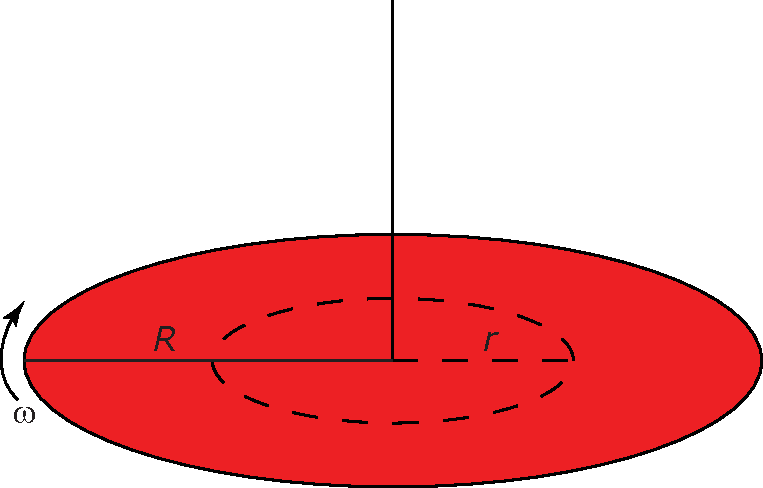
\includegraphics[width=0.35\linewidth]{fig/images/rotating_disk.pdf}
  \caption{A solid disk rotating about a centered, perpendicular axis with a constant angular velocity $\omega$}
  \label{fig:rotating_disk}
\end{figure}

Although each point of the disk is rotating with a constant angular velocity $\omega$, the linear velocity of each point is different. This can be easily determined using an understanding of rotation and time. The entire disk must undergo one complete revolution in time $\frac{2\pi}{\omega}$, but the distance that a point must travel in that time is dependent on its distance from the axis. For a point at a distance of $r$ from this axis, this distance is simply the circumfrence of a circle with radius $r$, or $2\pi r$. Using the formula $speed = \frac{distance}{time}$, the speed of this particle is defined by \cref{eq:v_and_w}. Thus, the rotating disk can actually be thought of as a combination of thin rings each consisting with particles moving at a unique velocity. 

\begin{equation}
v = \frac{2\pi r}{\frac{2\pi}{\omega}} = r\omega
\label{eq:v_and_w}
\end{equation}

For better generalization of this formula in instances where the velocity is not directly perpendicular to the axis of rotation, velocity can also be written as a cross product of the angular velocity vector (in the same direction as the axis of rotation) $\bm{\omega}$ and the position vector of the particle $\bm{r_i}$ as:

\begin{equation}
\bm{v_i} = \bm{\omega} \times \bm{r_i}
\end{equation}
and the angular velocity vector as:

\begin{equation}
\bm{\omega} = \omega \bm{k}
\end{equation}
where $\bm{k}$ is simply a unit vector in the direction of the rotational axis and $\omega$ is the magnitude of the angular velocity. Then, the velocity can simplified to:

\begin{equation}
\bm{v_i} = \omega |k \times \bm{r_i}|
\end{equation}

$|\bm{k} \times \bm{r_i}|$ is equivalent to the perpendicular distance between the point and the axis of rotation, which will be proved later. Using this value, we can utilize the traditional formula for kinetic energy to calculate the energy for a single rotating particle as:

\begin{equation}
R.K.E._i = \frac{1}{2}m_i\omega^2 |\bm{k} \times \bm{r_i}|^2
\label{eq:particle_rotational_energy}
\end{equation}

and the rotational energy for the entire body as:

\begin{equation}
R.K.E. = \sum_i \frac{1}{2}m_i\omega^2 |\bm{k} \times \bm{r_i}|^2
\label{eq:total_rotational_energy}
\end{equation}

To simplify this equation, the moment of inertia of a body is empirically defined as:

\begin{equation}
I = \sum_i m_i|\bm{k} \times \bm{r_i}|^2
\label{eq:total_moment_inertia}
\end{equation}

which for a single particle can be simplified to:

\begin{equation}
I = mr^2
\label{eq:simple_moment_inertia}
\end{equation}

where $r$ is the perpendicular distance from the particle to the axis.

The general formula for rotational kinetic energy can then be defined by \cref{eq:basic_rke} using two values, the rotational velocity $\omega$ and the moment of inertia $I$, which for a body rotating at a constant velocity about a fixed axis are constants (similar to $M$ and $v$ for traditional kinetic energy)~\parencite{Young_Freedman_Young_2020}.

\begin{equation}
R.K.E = \frac{1}{2}I\omega^2
\label{eq:basic_rke}
\end{equation}

Plugging in \cref{eq:simple_moment_inertia} and \cref{eq:v_and_w} to the equation for rotational kinetic energy shows that the final units remain the same as that for traditional kinetic energy presented in \cref{eq:basic_kinetic_energy}. Moment of inertias are also utilized to calculate angular momentum about a point which has many identical properties to traditional momentum, including conservation and collision governance. Using this information, I will derive moment of inertia formulas for a multitude of common bodies in motion.

\subsection{Vector Cross Products}

The formula for moment of inertia relies on the magnitude of a cross product. The general formula for the magnitude of a cross product is defined as~\parencite{Hass_Heil_Weir_2018}:

\begin{equation}
|\bm{u} \times \bm{v}| = |\bm{u}||\bm{v}|\sin{\theta}
\label{eq:cross_product}
\end{equation}

where $\theta$ is the angle between the two vectors.

This can be proved using basic vector rules:

\begin{gather*}
\text{Let } \bm{u} = \begin{bmatrix}u_1\\u_2\\u_3\end{bmatrix} \text{ and } \bm{v} = \begin{bmatrix}v_1\\v_2\\v_3\end{bmatrix} \\
\bm{u} \times \bm{v} = \begin{vmatrix}
\bm{i} & \bm{j} & \bm{j}\\
u_1 & u_2 & u_3 \\
v_1 & v_2 & v_3
\end{vmatrix} = \begin{vmatrix}
u_2 & u_3 \\
v_2 & v_3
\end{vmatrix}\bm{i} - \begin{vmatrix}
u_1 & u_3 \\
v_1 & v_3
\end{vmatrix}\bm{j} + \begin{vmatrix}
u_1 & u_2 \\
v_1 & v_2
\end{vmatrix}\bm{k} = \begin{bmatrix}u_2v_3 - u_3v_2\\u_3v_1 - u_1v_3\\u_1v_2 - u_2v_1\end{bmatrix}\\
\end{gather*}

Then, the squared-magnitude of the cross-product can be defined as:
\begin{align*}
|\bm{u} \times \bm{v}|^2 &= (\bm{u} \times \bm{v}) \cdot (\bm{u} \times \bm{v}) \\
&= (u_2v_3 - u_3v_2)^2 + (u_3v_1 - u_1v_3)^2 + (u_1v_2 - u_2v_1)^2 \\
&= u_2^2v_3^2 + u_3^2v_2^2 + u_1^2v_3^2 + u_3^2v_1^2 + u_1^2v_2^2 + u_2^2v_1^2 - 2(u_2u_3v_2v_3 + u_1u_3v_1v_3 + u_1u_2v_1v_2)
\end{align*}

We can also observe two other intriguing results:
\begin{align*}
(\bm{u} \cdot \bm{v})^2 &= (u_1v_1 + u_2v_2 + u_3v_3)^2 \\
&= u_1^2v_1^2 + u_2^2v_2^2 + u_3^2v_3^2 + 2(u_2u_3v_2v_3 + u_1u_3v_1v_3 + u_1u_2v_1v_2) \\
\end{align*}
\begin{align*}
(|\bm{u}||\bm{v}|)^2 &= (\sqrt{u_1^2 + u_2^2 + u_3^2}\sqrt{v_1^2 + v_2^2 + v_3^2})^2 \\
&= (u_1^2 + u_2^2 + u_3^2)(v_1^2 + v_2^2 + v_3^2) \\
&= u_2^2v_3^2 + u_3^2v_2^2 + u_1^2v_3^2 + u_3^2v_1^2 + u_1^2v_2^2 + u_2^2v_1^2 + u_1^2v_1^2 + u_2^2v_2^2 + u_3^2v_3^2
\end{align*}

By subtracting the second result from the third result, we can acquire the first result, leading to the formula:
\begin{align*}
|\bm{u} \times \bm{v}|^2 &= (|\bm{u}||\bm{v}|)^2 - (\bm{u} \cdot \bm{v})^2 \\
&= (|\bm{u}||\bm{v}|)^2 - (|\bm{u}||\bm{v}|\cos{\theta})^2 \\
&= (|\bm{u}||\bm{v}|)^2 - (|\bm{u}||\bm{v}|)^2\cos^2{\theta} \\
&= (|\bm{u}||\bm{v}|)^2(1 - \cos^2{\theta}) \\
&= (|\bm{u}||\bm{v}|)^2\sin^2{\theta}
\end{align*}

This result can then be square rooted, resulting in the initial theorem presented in \cref{eq:cross_product}. Because of this formula, the cross product between a unit vector and the position vector can also represent the perpendicular distance between the direction of the unit vector and the specific position. This premise is crucial, because it simplifies many moment calculations and is adopted for this investigation.

\subsection{Parallel Axis Theorem}

To calculate the moment of inertia for more complex bodies, the parallel axis theorem is often utilized to relate the moment of inertia about an axis passing through the center of mass of a body to a parallel axis at a distance $d$ from the central axis~\parencite{Abdulghany_2017}. \cref{eq:parallel_axis_formula} describes the theorem, where $I_{cm}$ is the moment of inertia through an axis passing through the center of mass, $M$ is the mass of the body, and $I'$ is the resultant moment of inertia through the parallel axis. This equation is applicable for any body, regardless of shape or dimensions.

\begin{equation}
I' = I_{cm} + Md^2
\label{eq:parallel_axis_formula}
\end{equation}

To prove this relationship, consider a lamina with mass $M$ located in the $X-Y$ plane whose center of mass is located at the origin as in \cref{fig:parallel_axis_lamina}. A general point $i$ is depicted and has coordinated $(x_i, y_i)$ and the parallel axis passes through $O$ which has coordinates $(a, b)$.

% !TEX root = ../math_ia.tex
\begin{figure}[H]
  \centering
  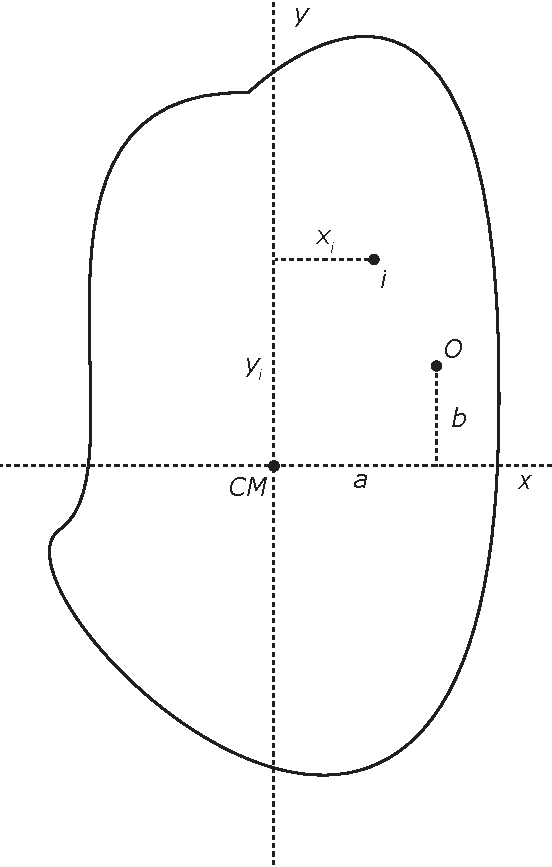
\includegraphics[width=0.25\linewidth]{fig/images/parallel_axis_lamina.pdf}
  \caption{A plain lamina in the $X-Y$ plane with its center of mass located at the origin}
  \label{fig:parallel_axis_lamina}
\end{figure} 

Because the center of mass is simply a weighted average of the mass of individual points on the lamina and the center of mass coincides with the origin, we can deduce:

\[x_{CM} = \frac{\sum_i m_ix_i}{M} = 0 \]
\[y_{CM} = \frac{\sum_i m_iy_i}{M} = 0 \]

Using the definition of moment of inertia for a particle and denoting the distance between point $i$ and point $O$ as $r_{iO}$, we can see $I_O = \sum_i m_i r_{iO}^2$. Using the distance formula, we have:

\[r_{iO}^2 = (x_i-a)^2 + (y_i-b)^2\]

Then,

\begin{align*}
I_O &= \sum_i m_i r_{iO}^2 \\
&= \sum_i m_i \left[(x_i-a)^2 + (y_i-b)^2\right] \\
&= \sum_i m_i \left[x_i^2 + a^2 - 2x_ia + y_i^2 + b^2 - 2y_ib\right]
\end{align*}

Now, using the deductions from the center of mass, the $2x_ia$ and $2y_ib$ terms can be removed, as $\frac{\sum_i m_ix_i}{M} = 0$ and $\frac{\sum_i m_iy_i}{M} = 0$, leaving:

\[I_O = \sum_i m_i (x_i^2 + y_i^2) + \sum_i m_i (a^2 + b^2) \]

Again, the distance formula (and the fact that the center of mass is located at the origin), allows us to see that $(x_i^2 + y_i^2)$ is simply equal to the square of the distance from point $i$ to the origin, or $r_i^2$, and $(a^2 + b^2)$ is equivalent to the square of the distance between point $O$ and the origin, or $d^2$. Then, we have:

\[I_O = \sum_i m_i r_i^2\ + \sum_i m_id^2\]

As we know that the first summation is equivalent to the moment of inertia about the center of mass (the origin) using \cref{eq:total_moment_inertia,eq:simple_moment_inertia}, and $d^2$ is constant, this simplifies to:

\[I_O = I_{CM} + Md^2\]

leaving the initial theorem as presented in \cref{eq:parallel_axis_formula}.
